\documentclass[11pt]{article}

\usepackage[utf8]{inputenc}
\usepackage[T1]{fontenc}
\usepackage[english, french]{babel} %français
\usepackage{amsmath}
\usepackage{amsfonts}
\usepackage{makeidx}
\usepackage{graphicx}
\usepackage[left=2cm,right=2cm,top=2cm,bottom=2cm]{geometry}
\usepackage{mathtools} %dcases
\usepackage{braket} %quantum mechanics
\usepackage[colorlinks=true, linkcolor=black, citecolor=black]{hyperref} % hyperlinks
\usepackage{tikz} % drawing in LaTeX
\usepackage{ dsfont } % hollow letters

% compile child documents using this preamble
\usepackage{subfiles}

% compile child files with separate preambles, and include them in the document
\usepackage{standalone}

% subfigure
\usepackage{caption}
\usepackage{subcaption} 

% the equal sign I use to define something
\newcommand{\define}{\ensuremath{ \overset{\text{def}}{=} }}

% differential element
\renewcommand{\d}[1]{\mathrm{d}#1}

% similar symbol with a limit underneath
\newcommand{\simlim}[2]{\ensuremath{ \underset{#1 \rightarrow #2}{\sim} }}

\newcommand{\om}{\ensuremath{\omega}}
\newcommand{\lb}{\ensuremath{\overline{\lambda}}}
\newcommand{\zb}{\ensuremath{\overline{z}}}

\title{\textbf{Fractal dimensions of quasicrystals \emph{via} a perturbative renormalization group.}}
\author{}
\date{}
\begin{document}

\selectlanguage{english}

\maketitle

%\abstract{}

We focus on tight-binding Hamiltonians on one-dimensional quasiperiodic tilings.
Notable examples include the Harper model, and the family of quasiperiodic Hamiltonians constructed by the cut and project method. 
Each of the latter is associated with an irrational number, $\alpha$.
It has the geometrical interpretation of the tangent of the angle between the projection axis and the direction of one of the basis vectors of the two-dimensional superlattice.
The Hamiltonian of such a model writes
\begin{equation}
	H^\alpha = \sum_i t^\alpha_i \left( \ket{i} \bra{i+1} + \ket{i+1} \bra{i} \right)
\end{equation}
where the jump amplitudes $t^\alpha_i$ can take two values $t_s$, $t_w$:
\begin{equation}
	t_i^\alpha = \begin{dcases*}
	t_w & when $i \bmod(1+\alpha) \geq \alpha$, \\
	t_s & otherwise.
	\end{dcases*}
\end{equation}
If we replace the irrational $\alpha$ by a rational approximation $\alpha_n = p_n/q_n$, the sequence of couplings is modified:
\begin{equation}
	t_i^{p_n/q_n} = \begin{dcases*}
	t_w & when $q_n i \bmod(p_n+q_n) \geq p_n$, \\
	t_s & otherwise,
	\end{dcases*}
\end{equation}
and we obtain a periodic system of period $p_n + q_n$. 
Thus, to a sequence of rationals $\{\alpha_n\}_n$ converging to $\alpha$ is associated in a natural way a sequence of periodic tight-binding Hamiltonians -- called approximants, converging to a quasiperidic Hamiltonian. We will call $H_n$ the $n^\text{th}$ approximant, generated by the rationnal $\alpha_n$.


Amongst all irrationals, the golden ratio and its inverse, $\omega = 2/(1+\sqrt{5})$, play a special role. They contain only the number 1 in their continued fraction expansion. In that sense, these two numbers are the hardest to approximate by rationnals. 
We thus expect the quasiperiodicity to have the most spectacular consequences when the irrational is taken to be the golden ratio or its inverse.

We restrict ourselves to the case $\alpha \leq 1$ (the other case being equivalent up the exchange of $t_s$ and $t_w$). As an example, we are going to chose $\alpha = \omega$. The tight-binding Hamiltonian resulting from this choice is called the Fibonacci Hamiltonian.
However, our results are general and apply to every Hamiltonian constructed by the cut and project method.

\section{Co-numbering, atoms and molecules.}

We consider a periodic approximant given by the rational $\alpha_n = p_n/q_n$. Later, we are going to specialize to the case of the Fibonacci Hamiltonian, but for the moment we wish to stay as general as possible.
We have already seen already that the integer
\begin{equation}
	i'_k = q_n k \bmod(p_n+q_n)
\end{equation}
determines the sequence of jump amplitudes. How does $i'_k$ changes when we jump from one site to the next, i.e. when we increase $k$ by one unit? It is easy to check that
\begin{equation}
	i'_{k+1} = \begin{dcases*}
	i'_k + p_n & when sites $k$ and $k+1$ are linked by $t_w$, \\
	i'_k + q_n & when sites $k$ and $k+1$ are linked by $t_s$.
	\end{dcases*}
\end{equation}
Thus, the sequence of $i'_k$ furnishes a natural renumbering of the sites, as was first noted by R. Mosseri \cite{Moss}. A generalization of this renumbering to higher dimensional quasicrystals can be found in \cite{MossSire}.
In the basis where sites are numbered using $i'$, up to a suitable shift of the origin, the Hamiltonian rewrites as a two-banded Toeplitz matrix:
\begin{equation}
	H_n = 
	\bordermatrix{ 
	 	& 1 	&	\ldots & & p_n	& &  \ldots &	& q_n &	& \ldots	&  \cr
    1 	& 0 		& \ldots & 0 & t_w & 0	& \ldots & 0 & t_s	& 0 		& \ldots		 \cr
    \vdots & & & & & \ddots	& & & & \ddots & \cr
    p_n & t_w \cr
    \vdots & & \ddots \cr
    q_n & t_s \cr
    \vdots & & \ddots \cr
     & 
    }
\end{equation}
The co-numbering allows to distinguish two classes of sites. We call \emph{molecular} the first $p_n$ and the last $p_n$ sites. We call \emph{atomic} the remaining $q_n - p_n$ sites.
Each molecular site is coupled to another molecular site by a $t_s$ coupling, and to an atomic site by a $t_w$ coupling. Thus, in the limit $t_w \ll t_s$, molecular sites form isolated diamtomic \emph{molecules}. 
On the other hand, the atomic sites are all coupled to two molecular sites by $t_w$ couplings. Thus, in the limit $t_w \ll t_s$, they form isolated \emph{atoms}.

Now, we focus on the particular case of the Fibonacci Hamiltonian. 
We take $p_n = F_{n-2}$, $q_n = F_{n-1}$ where $F_n$ is the $n^\text{th}$ Fibonacci number. Then, $\alpha_n = F_{n-2}/F_{n-1}$ indeed approximates the inverse golden ratio, so that we have constructed an approximant to the Fibonacci chain.
The $n^\text{th}$ Fibonacci approximant consists of a block of $F_{n-2} + F_{n-1} = F_{n}$ sites, repeated periodically. That block contain $F_{n-1} - F_{n-2} = F_{n-3}$ atoms and $F_{n-2}$ molecules (that is, $2F_{n-2}$ molecular sites).

Figure \eqref{fig:fib8} shows the molecules and atoms of the fifth Fibonacci approximant, together with the co-numbering of the sites.

\begin{figure}[htp]
	\centering
	\subfile{img/fibonacci_approximant.tex}
	\caption{The periodically repeated block of the fifth approximant to the Fibonacci chain. Weak couplings $t_w$ are represented by a single line, and strong couplings $t_s$ by a double line. Below each site is its co-numbered label.}
\label{fig:fib8}
\end{figure}

\section{Deflation and renormalization}

\subsection{Deflation, molecular and atomic chains.}
Besides the cut and project method, we can construct the Fibonacci chain by inflation.
We start from the trivial chain:
\begin{equation}
	C_0 = t_s
\end{equation}
and we apply repetively the \emph{inflation rule}
\begin{equation}
	r \define \begin{cases}
        t_{w} & \rightarrow t_w t_s \\
        t_s & \rightarrow t_w
      \end{cases}
\end{equation} 
on it to build new chains: $C_1 = r(C_0) = t_w$, $C_2 = r(C_1) = t_w t_s$, ... $C_n = r^n(C_0)$.
Then, perhaps up to a global circular permutation of the couplings, the infinite chain $C_n C_n C_n \dots$ is the sequence of couplings of the $n^\text{th}$ approximant.
Furthermore, we can define \emph{deflation rules} relating an approximant to a smaller one.
The \emph{molecular deflation rule}
\begin{equation}
	d_m = \begin{cases}
        t_{w} & \leftarrow t_s t_w t_w (t_s)\\
        t_s & \leftarrow t_s t_w (t_s)
      \end{cases}
\end{equation}
decimates all sites except molecular ones. Fig. \eqref{fig:mol_defl} examplifies the decimation operation.
Crucially, the deflated chain is again a Fibonacci chain. More precisely, the molecular deflation relates the approximant of size $n$ to the approximant of size $n-2$: $d_m(C_n C_n \dots) = C_{n-2} C_{n-2} \dots$.

\begin{figure}[htp]
	\centering
	\subfile{img/molecular_deflation.tex}
	\caption{The molecular deflation rule illustrated. Here we relate the fifth approximant to the third.}
\label{fig:mol_defl}
\end{figure}

Similarly, we can perform a decimation operation on all sites except atomic ones. We call such an operation an \emph{atomic decimation}.
Again, the deflated chain is also a Fibonacci chain.
The atomic decimation relates the approximant of size $n$ to the approximant of size $n-3$. 
Fig. \eqref{fig:at_defl} examplifies the procedure.

\begin{figure}[htp]
	\centering
	\subfile{img/atomic_deflation.tex}
	\caption{The atomic deflation rule illustrated. Here we relate the fifth approximant to the second.}
\label{fig:at_defl}
\end{figure}

\subsection{Renormalization}

We are now going to focus on the limit $t_w \ll t_s$, in which the disinction between atomic and molecular sites acquires its real meaning.
We define $\rho = t_w/t_s$. It will be our perturbative parameter.
The energies are at most of order $t_s$. As varying $t_s$ (while keeping $\rho$ fixed) simply amounts to rescaling the whole energy spectrum, we arbitrarily set $t_s = 1$. 

When $\rho = 0$, the atoms and the molecules decouple. The eigenstates are the molecular bonding and antibonding states, at energies $\pm 1$, and the atomic state at zero energy.
The spectrum is constituted of three infinitely degenerated levels.

When $\rho > 0$, $\rho \ll 1$, perturbation theory tells us that states inside each of the three degenerated levels weakly coupled to each other, thus raising the degeneracy.
Let us focus to begin with on atomic states. At first order, each atomic site is coupled to the neighbouring atomic sites.
Effectively, we can therefore work on the \emph{deflated} chain, with effective hopping amplitudes coupling atomic sites. Perturbation theory gives us the expression of the effective hopping amplitudes \cite{Niu1990}.
We find
\begin{equation}
	\begin{dcases}
	t^\text{atomic}_w &= \zb \rho\\
	t^\text{atomic}_s &= \zb,
	\end{dcases}
\end{equation}
with $\zb =\rho^2$.

Similarly, each molecular site is coupled to the neighbouring molecular sites. 
There is here a small subtlety. A molecule sits on two neighbouring sites. Say for example that that sites $i$ and $i+1$ on the chain form a molecule.
Then, by a change of basis, we can say that the molecule sits at the ``bonding'' and ``antibonding'' sites whose position is respectively given by the linear combination of the localized states $\ket{i} + \ket{i+1}$ and $\ket{i} - \ket{i+1}$.
It is natural to do that, because when $\rho = 0$ the molecular eigenstates are localized in this new basis.
At first order, the bonding sites couple to each other. 
This results in effective hopping amplitudes given by
\begin{equation}
	\begin{dcases}
	t^\text{bonding}_w &= z \rho\\
	t^\text{bonding}_s &= z,
	\end{dcases}
\end{equation}
with $z = \rho/2$. This also results in the appearance of an onsite potential, $V^\text{bonding}  = -1$. 
The antibonding sites similarly couple to each other, resulting in the same effective hopping terms, but in a different onsite potential, $V^\text{antibonding} = +1$.

To summarize, we have seen that we can formally separate the chain of the $n^\text{th}$ approximant into molecular and atomic chains.
In the limit $\rho \ll 1$, the Hamiltonian of the $n^\text{th}$ approximant decouples into the direct sum of three Hamiltonian: an atomic Hamiltonian living on the atomic chain, a bonding Hamiltonian living on the molecular chain, and an antibonding Hamiltonian also living on the molecular chain. 
Because the atomic and molecular chains are again Fibonacci chains (but of smaller lengths), we can relate these three Hamiltonians to Fibonacci Hamiltonians, with renormalized hopping terms and onsite energies.
We can summarize these results in an equation:
\begin{equation}
	H_n = \left( z H_{n-2} - 1 \right) \oplus \left( \zb H_{n-3} \right) \oplus \left( z H_{n-2} + 1 \right) 
\end{equation}

In the limit $n \rightarrow \infty$, the chain becomes quasiperiodic. As such, we expect its wavefunctions and its spectrum to be nontrivial, namely to exhibit multifractality.
We are going to try using the recursion relation we have on the Hamiltonians of the approximants to derive recursion relations on energies and wavefunctions. In this way, we hope to gain some insight on the form of the spectrum and of the wavefunctions in the limit $n \rightarrow \infty$.
From that, we hope to characterize the multifractality of the quasiperiodic chain by computing the fractal dimensions of its wavefunctions and of its spectrum.

\subsection{Renormalization paths, equivalence between energy labels and co-numbers.}

%The co-numbering naturally distinguishes between molecules and atoms.
%For the $n^\text{th}$ approximant, the first $p_n = F_{n-2}$ sites are the left part of a molecule. We will attach to these sites a label $m_l$. The next $q_n - p_n = F_{n-3}$ sites are the atomic sites, and we will label then $a$. The last $p_n = F_{n-2}$ sites are the right part of a molecule, we will label them $m_r$.
%We can repeat this procedure at the step $n-2$ for molecular sites, $n-3$ for atomic sites, until we reach the trivial state $n=1$ or $n=0$. 
%We see that there is a one-to-one mapping between the co-number of a site, $i$, and the sequence of labels $l_n l_{n-2/n-3} \dots l_s \dots$, where $l_s = m_l, a$ or $m_r$ is the label of the site at step $s$.

%In the perturbative picture, we can thus represent each state as a sequence of labels, which we call its \emph{renormalization path}. 
%We can plot these sequences on a trifurcating tree (fig. \eqref{fig:tree_states})

Since the Hamiltonian of an approximant is the direct sum of three Hamiltonians, the energy spectrum is split into three bands.
Specifically, the spectrum $\mathcal{S}_n$ of the $n^\text{th}$ approximant is the union of scaled version of the spectra at step $n-2$ and $n-3$:
\begin{equation}
\label{eq:recur_spectrum}
	\mathcal{S}_n = \left( z \mathcal{S}_{n-2} - 1 \right) \bigcup \left( \zb \mathcal{S}_{n-3} \right) \bigcup \left( z \mathcal{S}_{n-2} + 1 \right) 
\end{equation}
 
The upper band, associated to molecular bounding states, will be given a $+$  label.
The middle band, associated to atomic states, will be given a $0$ label, and the lower band , associated to molecular antibonding states will be given a $-$ label.
Repeating this labelling procedure recursively, we can assign to each energy level of the $n^\text{th}$ approximant a unique sequence of labels, which we call its renormalization path.
We can plot these sequences on a trifurcating tree (fig. \eqref{fig:tree_en}), as was pointed out in particular in \cite{KaluginKitaevLevitov} and \cite{Piechon95}.

\begin{figure}[htp]
\centering
    	\begin{tikzpicture}[scale=.7]
    		\newcommand{\orig}{-1.5}
    		\newcommand{\trans}{1.5}
    		\newcommand{\vertspac}{-2.}
    		\newcommand{\vertsize}{.5} % vertical spand of the rectangles
    		\newcommand{\del}{.2}
		\end{tikzpicture}
\caption{Trifurcating tree of energies.}
\label{fig:tree_en}
\end{figure}

\begin{figure}[htp]

\centering
\begin{subfigure}{.5\textwidth}
  \centering
  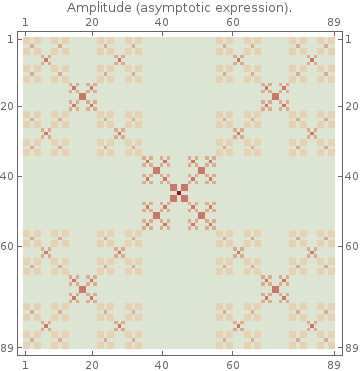
\includegraphics[width=.8\textwidth]{img/amplitude_asym.png}
  \caption{Amplitude, asymptoptic expression.}
  \label{fig:wf_idos_asym}
\end{subfigure}%
\begin{subfigure}{.5\textwidth}
  \centering
  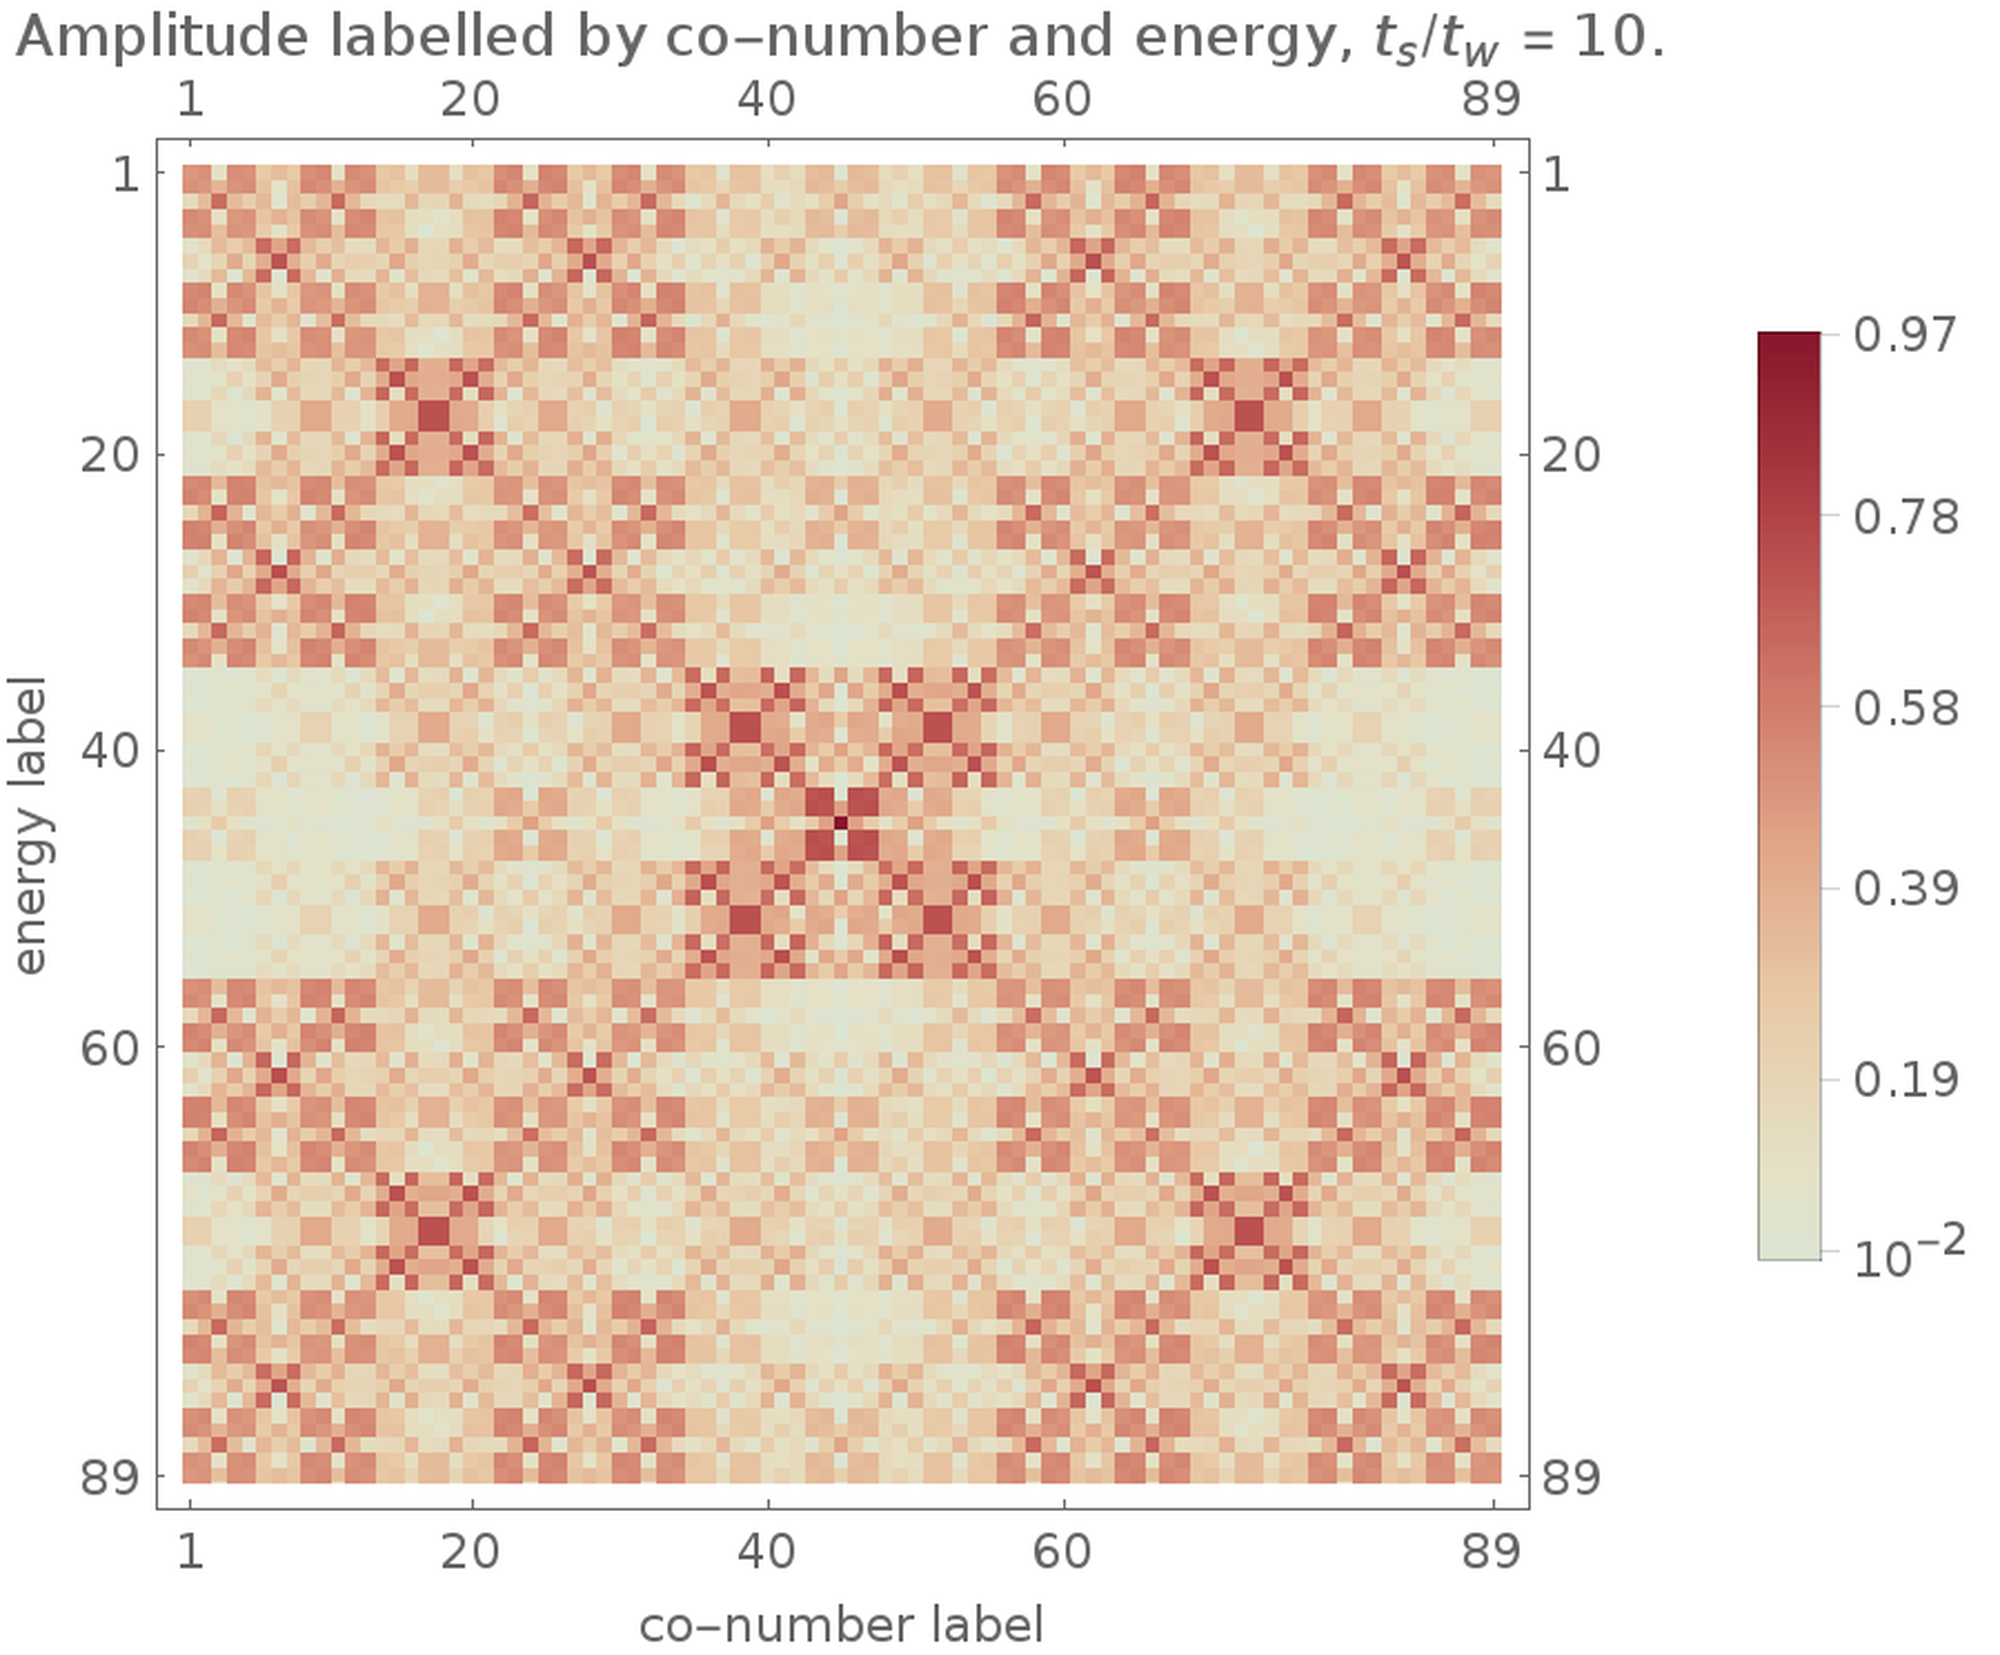
\includegraphics[width=1.\textwidth]{img/wf_idos.png}
  \caption{Amplitude, numerical expression.}
  \label{fig:wf_idos_num}
\end{subfigure} \\

\caption{The amplitude of the wavefunctions coefficients, ordered by co-numbering and energy. }
\label{fig:wf_idos}
\end{figure}

At step $n$, we can distinguish three types of sites: bonding sites, atomic sites and antibonding sites.
We label $+$ the bonding sites, $0$ the atomic sites and $-$ the antibonding sites.
Exactly as was done for energy levels, we can repeat this labelling procedure recursively, and assign to site level of the $n^\text{th}$ approximant a unique sequence of labels, which we call its renormalization path.

At first order in $\rho$, the state corresponding to a given energy level has a non-zero amplitude only at sites whose renormalization path match the one of the energy level.
Thus, in the limit $\rho \ll 1$ we are able to construct energy bands and eigenstates from the sole knowledge of their renormalization paths. 

This result has important consequences. In particular, it implies a symmetry between sites in co-numberig and energy levels labelled by increasing energy (fig. \eqref{fig:wf_idos}).

\section{Eigenstates renormalization}

At leading order in $\rho$ the renormalization of the eigenstates is trivial: an atomic eigenstate at step $n$ is just an eigenstate of the system at step $n-3$, while a molecular eigenstate is just an eigenstate of the system at step $n-2$, divided by a factor of $\sqrt{2}$ because we have two molecular clusters.

At this order, the recursion relation between energies \eqref{eq:recur_spectrum} makes it easy to find the fractal dimensions of the spectrum \cite{Piechon95} \emph{via} the implicit equation
\begin{equation}
	2 \omega^2 \zb^{-(q-1)D_q}+\omega^3 z^{-(q-1)D_2} = 0
\end{equation}
In particular, we find for the Hausdorff dimension
\begin{equation}
	D_0 = \frac{\log( \sqrt{2} -1 )}{\log \rho}
\end{equation}
Note that Damanik \& Gorodetski \cite{DamanikGorodetski} found the same Hausdorff dimension for the diagonal model, in the weak-coupling regime, using trace-map-based methods. Perhaps is there a mapping between the two?

Moreover, we can compute the fractal dimensions of the wavefunctions. We find
\begin{equation}
	D_q(i) = x_i \frac{\log 2}{\log \tau}
\end{equation}

To go beyond the leading order -- where the interesting physics lies! -- we have to consider overlap between atoms and molecules. We are now going to suppose that atomic eigenstates have non zero presence probability on molecules, an vice-versa.

However, since for example an energy $E$ of the atomic cluster at step $n$ corresponds to an energy $E/\zb$ at step $n-3$, we still hope to relate the amplitudes of the atomic eigenstate if energy $E$ on atomic sites, to the amplitude of the eigenstate of energy $E/\zb$ at step $n-3$. Specifically, we are going to assume that they are simply related by scaling factor:
 \begin{equation}
\label{eq:renorm_a}
	\psi_i^n(E) = \sqrt{\lambda} \psi^{n-3}_{d_a(i)}(E/\bar z)
\end{equation}
where $d_a(i)$ is the new numbering of the site $i$ after an atomic deflation operation.

We can easily compute this factor perturbatively (see appendix \eqref{app:renorm}). We find
\begin{equation}
	\bar \lambda(\rho) = \frac{1}{1+2\rho^2} +\mathcal{O}(\rho^4).
\end{equation}
Now, knowing the amplitude of this atomic eigenstates on neighbouring \emph{molecular} sites is easy enough. We find
\begin{equation}
	\begin{cases}
	\psi^n_{i\pm1} &= \phantom{-}0 \\
	\psi^n_{i\pm2} &= - \rho \psi^n_i \\
	\psi^n_{i\pm3} &= \phantom{-}0 \\
	\psi^n_{i\pm4} &= \phantom{-}\rho^2 \psi^n_i
	\end{cases}
\end{equation}
at leading order.

\section{Fractal dimensions in the perturbative limit}

\section{Relations between fractal dimensions and universality}

\newpage
\appendix

\section{Renormalization factors of atomic and molecular eigenstates}
\label{app:renorm}

In this appendix, we derive the expression of the renoralization factors $\lambda$ and $\bar \lambda$ of the molecular and atomic eigenstates.

\subsection{Atomic eigenstates}

Let $\ket{\psi(E)}$ be an eigenstate for an energy $E$ belonging to the atomic energy cluster, at step $n$.
At first order, $\ket{\psi(E)}$ is an eigenstate of $\zb H_{n-3}$, with the sites rearranged on the $n^\text{th}$ approximant.
Therefore, at first order $\ket{\psi(E)}$ is only nonzero on some atomic sites of the $n^\text{th}$ chain. Let $i$ label one of these sites.

The fact that $\ket{\psi(E)}$ is an eigenstate of $\zb H_{n-3}$, with the sites rearranged on the $n^\text{th}$ approximant translates into the equation
\begin{equation}
\label{eq:renorm_a_first}
	\psi_i(E) = \psi_{d_a(i)}(E/\bar z),
\end{equation}
where $d_a(i)$ is the new numbering of the site $i$ after an atomic deflation operation.

Now, at the next order, some of the intensity, that was at first order concentrated only on some atomic sites, ``leaks'' on the molecular sites neighbouring these atomic sites. 
This translates into the fact that the intensity on these atomic sites is reduced by a factor $\lb$.
So, at second order, equation \eqref{eq:renorm_a_first} becomes
\begin{equation}
\label{eq:renorm_a}
	\psi_i(E) = \sqrt{\lb} \psi_{d_a(i)}(E/\bar z).
\end{equation}
To determine $\lb$, we just have to compute how much intensity has leaked out of site $i$.

\begin{figure}[htp]

\centering
\begin{subfigure}{.5\textwidth}
  \centering
  \includestandalone[width=.82\textwidth]{img/local_environment_atoms1}
  \caption{Atomic site surrounded by strong and weak effective couplings.}
  \label{fig:atom1}
\end{subfigure}%
\begin{subfigure}{.5\textwidth}
  \centering
  \includestandalone[width=1.\textwidth]{img/local_environment_atoms2}
  \caption{Atomic site surrounded by two weak effective couplings.}
  \label{fig:atom2}
\end{subfigure} \\

\caption{The two types of local environments of an atomic site. }
\label{fig:energyconf1}
\end{figure}

The atomic site $i$ we consider can either be surrounded by one weak effective bond (fig. \eqref{fig:atom1}), or by two effective weak bonds (fig. \eqref{fig:atom2}).
In both cases, it is straighforward to compute, at leading order in $\rho$, the fraction of the amplitude at site $i$ who is transferred to neighbouring molecular sites.
Note that destructive interferences result in half the molecular sites being unaffected at leading order.

As we already said, at first order in $\rho$, the amplitude in concentrated at site $i$. We call $I$ the intensity at this site: $I=|\psi_i|^2$. 
At second order in $\rho$, the intensity $I$ has spread out at neighbouring molecular sites, and therefore the intensity at site $i$ is attenuated by a factor $\lb$. We have
\begin{equation}
	\lb I ( 1 + 2\rho^2 + \mathcal{O}(\rho^4)) = I,
\end{equation}
And thus
\begin{equation}
	\lb = \frac{1}{1+2 \rho^2} + \mathcal{O}(\rho^4).
\end{equation}

\subsection{Molecular eigenstates}

\newpage

\bibliography{fractal_dimensions_quasicrystals.bib}{}
\bibliographystyle{plain}
\end{document}